% !TEX root = ../../Build/main.tex
% ###################################################################
% Copyright (c) 2018, Marc De Graef 
%  Editors: A.D. Rollett & M. De Graef
% All rights reserved.
%
% Licensed under the Creative Commons CC BY-NC-SA 4.0 License, 
% hereafter referred to as the "License"; you may not use this 
% document except in compliance with the License. You may obtain 
% a copy of the License at 
%     https://creativecommons.org/licenses/by-nc-sa/4.0/legalcode 
% Unless required by applicable law or agreed to in writing, all 
% material distributed under the License is distributed on an 
% "AS IS" BASIS, WITHOUT WARRANTIES OR CONDITIONS OF ANY KIND, 
% either express or implied. See the License for the specific 
% language governing permissions and limitations under the License.
% ###################################################################

% ###################################################################
% The following lines are to be uncommented or edited as needed 

%\corechapter{Yes}
%     uncomment this line only if this chapter is a core/foundational chapter;
%     for a core chapter a "Core" label will appear on the top left above the chapter title.

\chapterauthor{Marc De Graef, Carnegie Mellon University}
%     this will appear in a secondary header below the chapter title.

% All figures are stored in the src/MaterialProperty/eps folder and must be of the *.eps type. 
\renewcommand{\chaptergraphicspath}{../src/MaterialProperty/eps/}

\chapterimage{MATPRPheader.pdf}
%     replace \noheaderimage by the chapter header image file name (without .eps extension).
%     Chapter header images must be 2480 x 1240 pixels with 300dpi, RGB format.
\renewcommand{\chabbr}{MATPRP}
% ###################################################################

\chapter{What is a Material Property?\OClabel{MaterialProperty}}

\begin{messagebox}{What you will learn in this chapter}{ocre}{\icinfo}{white}
\begin{itemize}
	\item A formal definition of a material property (\OCref{matprop})
	\item The mechanics of coordinate transformations (\ref{sec:transformations1})
	\item A formal definition of tensors (\ref{sec:tensors})
	\item Important material property tensors (\ref{sec:materialtensors})
\end{itemize}
\end{messagebox}

\section{Introductory Remarks}

\begin{floatingfigure}[r]{3.2in}
\centering
{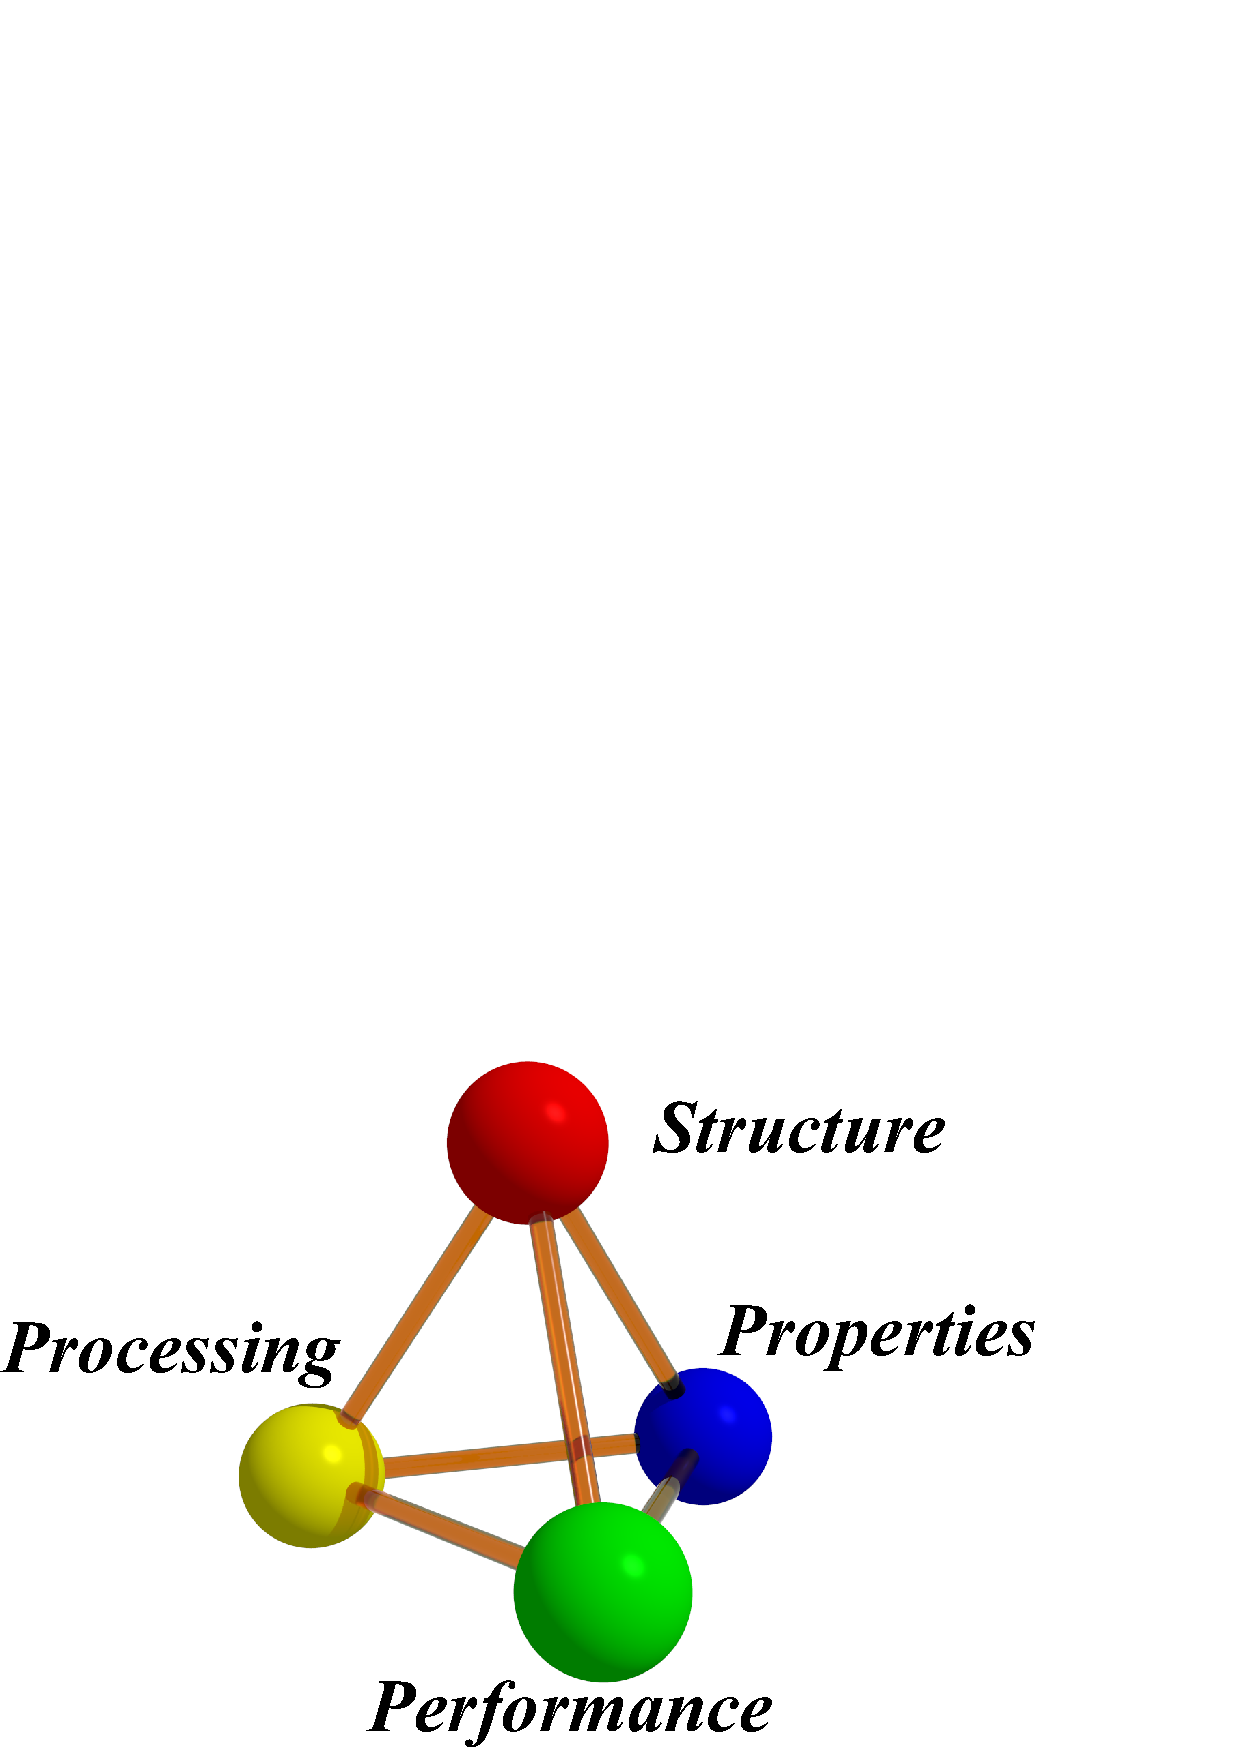
\includegraphics[width=3.0in]{tetrahedron.pdf}}
{\caption{\OClabel{tetrahedron}\small Graphical representation of the materials paradigm as a tetrahedron.}}
\end{floatingfigure}
\noindent It is not uncommon for the material scientist to describe their discipline in terms of a \indexit{tetrahedron}.  Each corner of the materials tetrahedron (Fig.~\OCref{tetrahedron}) represents one of the four cornerstones of the field: \textit{Microstructure, Properties, Processing}, and \textit{Performance}. Many materials scientists/engineers believe that optimization of material properties and performance through judicious control of processing parameters to obtain the desired microstructure is the central paradigm of the discipline.  Blacksmiths represent the original (empirical) practitioners of this approach; they vary the microstructure of steels by varying their heat treatment in order to affect their mechanical properties.  In the present day, we control the doping of semiconductors to make quantum dots, resulting in highly efficient light emitting diodes; this is phase separation\index{phase separation} to make a two-phase structure in which the size of the approximately spherical particles of one phase is small enough that quantum effects become important.

On the one hand, we have material properties, such as: strength, toughness, formability, conductivity, corrosion resistance, piezoelectricity, , magnetic permeability, $\ldots$ On the other hand we have microstructural features, such as: grain size, grain shape, phase structure, composite structure, chemical composition (alloying), crystal structure, defect structure (e.g., porosity), and many others. It is the primary goal of this collection of chapters to explicitly describe the links between properties and microstructure; in other words, this text focuses on the many connections between the red and blue spheres in Fig.~\OCref{tetrahedron}.\\  

\subsection{Microstructure\OClabel{microstructures}}
\indexit{Microstructure} refers to the internal structure of a material, at various length scales.  Biology was revolutionized when \indexit{Leeuwenhoek} and others started to use optical microscopes to look at the internal structure of plants.  They were able to relate many characteristics of plants to their cell structure, for example.  Similarly, in what is now the materials field, \indexit{Sorby} was one of the first to make cross-sections of materials such as iron and examine them in the microscope, so that he could relate properties to structure.  Microstructure originally meant the structure inside a material that could be observed with the aid of an optical microscope; in the metric system, with its prefixes for units, the micrometer ($1$ $\mu$m $= 10^{-6}$ m) happens to correspond roughly to the wavelength of light.  Light obviously is used to form images in a light/optical microscope.  Thus, microstructure has come to be accepted to cover those elements of structure with a length scale on the order of $1$ $\mu$m.  Given microstructure at the $\mu$m scale, naturally some refer to \textit{nanostructure}\index{nanostructure} at the nm ($=10^{-9}$ m) scale.  Many important material properties are determined at the atomistic length scale. The continuum scale means, in the context of engineering, length scales large enough that materials can be treated as having homogeneous properties.

Most observable elements of microstructure are discontinuities, or \indexit{defects}, in the material.  Some of the most important defects include:
\begin{itemize}
	\item \indexit{grain boundaries}  are discontinuities in the crystal lattice and correspond to abrupt changes in the orientation of the crystal lattice;
	\item \indexit{phase boundaries}  are discontinuities in composition and, commonly, in crystal structure;
	\item \indexit{dislocations}  are local discontinuities in the lattice translational periodicity; they require observations in the nanoscale regime but their combined effect becomes noticeable at the microstructure level;
	\item \indexit{point defects} (very difficult to observe!)  are missing atoms (vacancies)\index{vacancy} or extra (interstitial)\index{interstitial} atoms; they require high resolution transmission electron microscopes to detect their presence but their effect can also be felt at the microstructure level.
\end{itemize}

Direct observation of microstructures requires us to make \textit{images}. In order of increasing effort, the standard methods are (1) \indexit{optical microscopy} (OM), (2) \indexit{scanning electron microscopy} (SEM),  (3) \indexit{scanning probe microscopy} (SPM), and (4) \indexit{transmission electron microscopy} (TEM).  Microscopies that rely on topographic contrast require specimen preparation in order to reveal the microstructure.  Metallography/ceramography\index{metallography}\index{ceramography} is the art of specimen preparation for microscopy.  The aim in specimen preparation is always to maximize contrast for the microstructural elements of interest while minimizing image artifacts.\footnote{Reminder: not all imaging methods require topographic relief.  Channeling contrast in the SEM uses variations in crystallographic orientation to affect image brightness giving a gray-scale image of grain structure, for example.}

It is essential to quantify microstructure in order to be able to predict properties quantitatively; what needs to be quantified depends on the property, i.e., what question is asked of the material. Examples of quantitative microstructural parameters are: grain size, void fraction, second phase particle size, $\ldots$.  Before discussing specific techniques, we must point out that the discipline of \indexit{stereology} is essential.  Most real materials are three dimensional, whereas most characterization methods provide information from either a planar section or from a surface. Even TEM requires thin foils (about $0.1$ $\mu$m thick or less). Therefore, some more sophisticated analysis is required to extract the true 3D quantities of interest. Modern materials characterization techniques include approaches to reconstruct the full 3D microstructure of a material, and this can be done at various length scales:

\begin{itemize}
\item \textit{Atomic scale}:  the  3-D  atom probe\index{3D atom probe} \cite{seidman2000a,miller2004a,hono2005a} can generate maps of the locations of large numbers ($10^6$--$10^8$) of individual atoms in a relatively short time. The technique relies on field evaporation of individual atoms from a sharp tip placed in a strong electric field, and subsequent position and mass sensitive detection of these atoms.  This technique is limited to volumes of a few hundred cubic nanometers, and is very demanding in terms of sample preparation, but results in the ultimate resolution, since each atom is identified with respect to both chemistry and position.

\item \textit{``several cubic microns''}:  Focused ion beam (FIB)\index{focused ion beam}\index{FIB} serial sectioning techniques \cite{dunn1999a,uchic2006a} are used to analyze the 3-D  structure of polycrystalline sample with potentially complex phase mixtures.  When combined with \indexit{electron backscatter diffraction} and \indexit{energy dispersive x-ray spectroscopy}, orientational and chemical information can be acquired at the same time.  This technique is typically limited to a few hundred cubic microns.  More recently, \indexit{femto-second laser ablation} \cite{Echlin2015} has been used to remove larger volumes of material at a much faster rate.

\item \textit{``several cubic millimeters''}: Automated serial sectioning methods based on milling \cite{alkemper2001a} or standard metallography \cite{spowart2003a} can generate  3-D  data from macroscopic samples. Combining these approaches  with \indexit{Laue diffraction} and \indexit{x-ray fluorescence} allows for the near-simultaneous acquisition of chemical and orientational information.
\end{itemize}

\subsection{Properties}
\OClabel{properties}

A material's \indexit{properties} are those measurable characteristics that determine how the material responds to a variety of external stimuli; we will formalize this statement in section~\OCref{matprop}. Broad property categories and specific examples in each category include:
\begin{itemize}
\item \indexit{mechanical properties}: strength, hardness, ductility, toughness, fatigue resistance;
\item \indexit{thermal properties}: conductivity, heat capacity, thermal expansion;
\item \indexit{electrical and magnetic properties}: conductivity, resistivity, ferromagnetism, superconductivity, band gap;
\item \indexit{optical properties}: transparency, reflectivity, photoluminescence;
\item \indexit{chemical properties}: corrosion resistance, oxidation behavior, reactivity.
\end{itemize}

We distinguish between properties that are \indexit{intrinsic} and \indexit{extrinsic}. Intrinsic properties are generally determined by the crystal structure (i.e., the 3D arrangement and types of atoms) and in many cases they can be computed/predicted directly from the atomic arrangements using physics-based arguments, in particular quantum-mechanical models.  The electronic \indexit{band gap} of a material is  a typical example of an intrinsic property; it is fundamental to the particular crystal structure and represents the minimum energy needed to promote an electron from the valence band to the conduction band, thereby determining whether the material is an insulator, a conductor, or a semiconductor.  \textit{Ductility}\index{ductility} is an example of an extrinsic property since it depends in a very sensitive way on microstructural parameters, such as the grain size, or the rate at which the material is deformed (i.e., the \indexit{strain rate}).  In general, such extrinsic properties are much more difficult to predict since they depend on many factors that themselves may be difficult to quantify, and improving one extrinsic property, say strength, may have a negative effect on another property, in this case ductility.  The often complex and counter-acting dependencies between microstructure and (extrinsic) properties make it necessary to systematically approach material properties by starting from the single crystal state, and then gradually incorporating the actual microstructural aspects by means of appropriate averaging procedures, which represents a very active area of research.

\subsection{Processing}
\OClabel{processing}

Processing describes not only how we make a material (e.g., by solidification from a melt pool) but also how we subsequently modify the material's microstructure, for instance via thermal annealing or plastic deformation, both belonging to the category of \indexit{thermomechanical processing} techniques.    Each material class (metals, ceramics, polymers, $\ldots$) comes with its own set of specialized processing techniques, but the common goal of all material processing techniques is to achieve a microstructure that will satisfy all performance criteria or metrics (see next section).  

\begin{itemize}
	\item \textit{Metals}: 

	\item \textit{Ceramics}: 

	\item \textit{Polymers}: 
\end{itemize}

% and it is the primary way we control microstructure. Every processing step, whether heating, cooling, deforming, or applying energy� affects the arrangement of atoms and the evolution of microstructure. In metals, solidification from the melt establishes the initial grain structure; plastic deformation by rolling or forging introduces dislocations; subsequent heat treatments can reorganize those dislocations and change phases.

%Processing is not limited to traditional metallurgy. In ceramics, careful control of sintering temperature and atmosphere determines porosity and grain growth. In polymers, extrusion and drawing can align chains and improve strength. In electronic materials, epitaxial growth techniques deposit atomically precise thin films. More recently, additive manufacturing methods, such as laser powder bed fusion, are offering unprecedented control by  printing parts layer by layer. A key teaching point is that processing is a lever: by changing it, we can intentionally engineer microstructures, and therefore tune material properties.


\subsection{Performance}
\OClabel{performance}

Performance takes the discussion out of the lab and into the real world. It asks the question: How does the material actually behave in service, under realistic conditions and over long time scales? A material may exhibit excellent tensile strength in a simple test, but if it corrodes rapidly in a marine environment, its performance as a structural material for ships will be poor. Similarly, a ceramic may have outstanding hardness, but if it is too brittle, it cannot perform well in an application involving repeated impact.

Performance thus integrates not just the intrinsic properties of the material but also the environment, loading conditions, time, and cost. Engineers must consider fatigue (failure after many cycles of stress), creep (slow deformation at high temperature), wear, corrosion, and radiation damage. Performance also includes economic and societal factors, whether the material is sustainable, affordable, and available at scale.

In teaching, performance is often presented as the closing loop of the MSE framework. Microstructure is tailored by processing, which defines properties, which then dictate performance. This cycle emphasizes that materials are not just studied for their own sake but for their essential role in enabling technologies jet engines, medical implants, solar cells, bridges, and countless others.


\section{Definition of a Material Property}
\OClabel{matprop}

\begin{messagebox}{Important Section}{ocre}{\icattention}{black}
In this section you will learn a formal definition of what a material property is.  Later on in this chapter we will introduce many examples.
\end{messagebox}

Although it is difficult to provide a general abstract description of a material property, valid for all possible properties, it is instructive to think of a material property as \textit{the link between an external influence and the material's response to that influence}.  If we denote the external influence by $\mathcal{F}$ ($\mathcal{F}$ stands for \underline{F}ield or \underline{F}orce) and the material \underline{R}esponse or \underline{R}eaction by $\mathcal{R}$, then in the most general sense the relation between the two is given by
\begin{equation}
	\mathcal{R}=\mathcal{R}(\mathcal{F}),\label{eq:rf}
\end{equation}
or, put in words, the material response is a function of the externally applied field.  It is one of the tasks of a materials scientist to figure out and understand what that response function looks like.

We know from calculus that, for ``well-behaved'' functions, we can always expand the function into powers of its argument. For equation~(\ref{eq:rf}) above, the \indexit{Taylor expansion} around $\mathcal{F}=0$, i.e., the \indexit{McLaurin series}, is given by:
\begin{align}
	\mathcal{R}&=\mathcal{R}_0 + 
	\frac{1}{1!}\left.\frac{\partial\mathcal{R}}{\partial\mathcal{F}}\right 
	\vert_{\mathcal{F}=0}\!\!\!\!\mathcal{F} + 
	\frac{1}{2!}\left.\frac{\partial^2\mathcal{R}}{\partial\mathcal{F}^2}\right 
	\vert_{\mathcal{F}=0}\!\!\!\!\mathcal{F}^2 + 
	\frac{1}{3!}\left.\frac{\partial^3\mathcal{R}}{\partial\mathcal{F}^3}\right 
	\vert_{\mathcal{F}=0}\!\!\!\!\mathcal{F}^3 + \ldots \nonumber\\
	&= \mathcal{R}_0 +
	\sum_{n=1}^{\infty}\frac{1}{n!}\left.\frac{\partial^n\mathcal{R}}{\partial\mathcal{F}^n}\right 
	\vert_{\mathcal{F}=0}\!\!\!\!\mathcal{F}^n,
	\label{eq:expansion}
\end{align}
where $\mathcal{R}_0 = \mathcal{R}(0)=\mathcal{R}\vert_{\mathcal{F}=0}$ describes the ``state'' of the material at zero field.  There are two possibilities for $\mathcal{R}_0$:
\begin{enumerate}
	\item $\mathcal{R}_0=0$: in the absence of an external field ($\mathcal{F}=0$), there is no permanent (or \indexit{remanent}) material response.  For example, if the external field is an applied stress, and the material response is a strain, then at zero stress there is no strain (assuming linear elasticity).  Or, if the applied field is an electric field, and the response is an electrical current, then at zero field, no current flows (unless the material is in a superconducting state).
	
	\item $\mathcal{R}_0\neq 0$: in the absence of an external field ($\mathcal{F}=0$), there is a permanent material response.  For example, in a ferromagnetic material the magnetization is in general different from zero, even at zero applied field (i.e., a permanent magnet).  
\end{enumerate}

If we truncate the series after the second term (i.e., we ignore all derivatives of $\mathcal{R}$ except for the first one), then the expression for $\mathcal{R}$ becomes rather simple:
\begin{equation}
	\mathcal{R}=\mathcal{R}_0 + 
	\left.\frac{\partial\mathcal{R}}{\partial\mathcal{F}}\right 
	\vert_{\mathcal{F}=0}\!\!\!\!\mathcal{F} =\mathcal{R}_0 + 
	\mathbf{P}\mathcal{F}\quad\mbox{ with }\quad \mathbf{P}\equiv\left.  
	\frac{\partial\mathcal{R}}{\partial\mathcal{F}}\right\vert_{\mathcal{F}=0.
	}
\end{equation}
This is a \textit{linear} relation between the applied field and the response, and this relation becomes a proportionality between applied field and response when $\mathcal{R}_0=0$.  The quantity $\mathbf{P}$ is a \textit{material property}.\index{material property}  Ignoring the higher order derivatives of $\mathcal{R}$ is generally known as the \textit{linear approximation}.\index{linear approximation}  This approximation considerably simplifies the math and for many purposes it is a useful and accurate approximation.

Since the external field $\mathcal{F}$ is often a vector quantity (e.g., the electric field $\mathcal{F}=\mathbf{E}$) and the response can also be a vector (e.g., the current density $\mathcal{R}=\mathbf{j}$) it is clear that the material property $\mathbf{P}$ is not always going to be described by a single number.  Instead, the material property can become a vector itself, or even a higher order mathematical quantity known as a \indexit{tensor}; nearly all of the interesting and useful material properties are represented by tensors, in particular for single crystals but also in polycrystalline materials.  For now, think of a tensor as an array of numbers with a set of special properties; in Chapter~\OCref{tensors} the concept of a tensor is described in substantial detail.  Without going into the details at this time, we can state that, in general, a material property is represented by a \textit{matrix} of numbers; this can be a column vector, a $3\times 3$ matrix or even a higher dimensional array.  A combination of thermodynamic (or intrinsic) symmetry and the crystallographic symmetry of the material determines which of those numbers can be different from zero, and which \textit{must} be zero.  

If the series expansion in equation~(\ref{eq:expansion}) is truncated after the third term, then it is said that the material behaves in a non-linear way.  The relation can then be written as:
\begin{equation}
	\mathcal{R}=\mathcal{R}_0 + \mathbf{P}\mathcal{F} + 
	\mathbf{P}_2\mathcal{F}^2.
\end{equation}
$\mathbf{P}_2$ is a \textit{non-linear} material property.  Crystallography and symmetry theory can again be used to examine the relations between the components of $\mathbf{P}_2$.  
	
There are several material properties for which it is impossible to truncate the Taylor expansion of equation~(\ref{eq:expansion}) after just a few terms, and many or all terms must be used. For those properties, it is customary to use equation~(\ref{eq:rf}), with some appropriate mathematical function $\mathcal{R}$. In that case, equation~(\ref{eq:rf}) represents a so-called \indexit{constitutive law} or \indexit{constitutive relation}.  Sometimes, physical arguments can be used to find the precise form of the function, in other situations empirical or phenomenological relations may be needed.

One can also express the \textit{energy content} of a material in terms of the externally applied field(s); \textit{thermodynamics}\index{thermodynamics} then provides the means and rules to determine how the energy of a solid/liquid/gas changes when the external conditions change.  Thermodynamics often assumes that a material system is \textit{homogeneous} and \textit{isotropic} (see below) and then makes quite general statements about its behavior in various external fields.  Symmetry becomes important whenever a thermodynamic function depends on the gradient of a property; in such cases, symmetry theory can determine the possible mathematical expressions that will correctly describe this property.  There is thus an intimate relation between the symmetry of a material and its thermodynamic properties.  Whereas symmetry theory determines which elements of a property matrix must be zero, thermodynamics can be used to derive additional restrictions on the non-zero elements (e.g., some elements can only be positive, or certain elements must always be smaller than others, etc.)  

Every material property has a number of characteristics\footnote{We could call them \textit{properties} but it is a bit confusing to talk about the properties of a property.} which are of fundamental importance: \textit{homogeneity, anisotropy} and \textit{symmetry}; let us take a brief closer look at each of these concepts.

\subsection{Homogeneity}
\OClabel{homogeneity}

There are several length scales at which we can make observations on a material.  Macroscopic measurements are considered to be those measurements that are performed over distances many times larger than the interatomic distance, e.g.\
\begin{eqnarray}
	\mbox{length : }&&L \gg a; \nonumber\\
	\mbox{surface : }&&S \gg a^{2};\\
	\mbox{volume : }&&V \gg a^{3},\nonumber
\end{eqnarray}
where $a$ is of the order of the interatomic distance.  The majority of objects with which we deal in everyday life are composed of several different \textit{materials}: metals, plastics, wood, brick, and many others.  At the macroscopic level, most of those materials may appear to consist of only one piece.  However, when we use a microscope to zoom in on the details, we can often observe that the material is made up of small \textit{grains}.  Each of those grains is an individual crystal, usually with a rather irregular shape.  When we zoom in even further, we can observe the \textit{crystal lattice}, which shows a regular arrangement of atoms.  If a material consists of many grains in more or less random orientations, then we refer to that material as \textit{poly-crystalline}.  If the complete object is formed by only one grain, then that object is a \textit{single crystal}; many gems are single crystals.  It is customary to concentrate first on the properties of single crystals, and subsequently determine how a deviation from the single crystal state affects those properties.  To obtain a deeper understanding about the way materials work it is necessary to start at the microscopic or \textit{crystallographic} level and work our way up to real materials.

A crystalline substance is \textit{homogeneous}\index{homogeneous} when all physical (e.g.\ optical, mechanical, etc.)  and physicochemical (e.g.\ solubility of surface, adsorption, etc.)  properties are the same for volume (or surface) elements at different locations in the substance.  If a material point is denoted by the coordinate vector $\mathbf{r}$, then the mathematical statement of homogeneity of a property $\mathbf{P}$ becomes :
\begin{equation}
	\mathbf{P}(\mathbf{r}\,)=\mathbf{P}(\mathbf{r}+\mathbf{r}^{\,\prime})
\end{equation}
where the points $\mathbf{r}$ and $\mathbf{r}^{\,\prime}$ are separated by a (random) macroscopic distance.  The property $\mathbf{P}$ can be a scalar (heat capacity, density, etc.), a vector (polarization, magnetization, etc.)  or a higher order quantity known as a tensor (elastic moduli, magnetic susceptibility, etc.). \textit{Homogeneity} thus requires that a material property be independent of the location in the material where it is measured.  If a property \textit{does} depend upon location, then it is said that the property is \indexit{heterogeneous}.  For instance, a natural sapphire (Al$_2$O$_3$) crystal may contain Cr atoms; if the distribution of Cr atoms is homogeneous throughout the sample, then the color of the crystal will be independent of location.  However, if one side of the crystal contains more Cr than the other side, then there is a \textit{compositional gradient} across the sample, and the color may vary with location.  For many materials applications homogeneity is a strict requirement; for instance, for the cables used in suspension bridges, we want the mechanical properties to be the same along the length of the cables. For many other applications gradients or fluctuations are required;  for instance, if a semiconductor device were chemically homogeneous, it would completely fail to function.

% idea: add figure showing color gradations in tourmaline

\subsection{Anisotropy}
\OClabel{anisotropy}

A homogeneous property can be either isotropic or anisotropic in a single crystal.  If a property is the same in every direction, then that property is said to be \textit{isotropic},\index{isotropic} otherwise it is \textit{anisotropic}.\index{anisotropic}  Every isotropic homogeneous quantity must necessarily be described by a \textit{scalar}.  The most interesting properties are usually those which are direction dependent.  We will see later on that the mathematical quantity known as a tensor is perfectly suited for the description of anisotropic behavior.  Examples of properties which may depend upon direction include thermal conductivity, dielectric and magnetic susceptibilities, elastic moduli, and so on.  It is important to note that an anisotropic property in a single crystal can become isotropic in a poly-crystalline material, since all crystal orientations may be simultaneously present in the poly-crystal.

\subsection{Symmetry}
\OClabel{symmetry}

Symmetry is one of the more fundamental properties of crystalline matter.  Apart from color, it is also in many cases the most ``eye-catching'' aspect of a natural crystal.  One can introduce the concept as follows: take an arbitrary object and determine if there is a way to ``move'' the object into another orientation in such a way that the initial and final configurations are indistinguishable.  The specific ways of ``moving'' an object into \textit{self-coincidence} represent the symmetries of that object.  Enumeration of the different symmetry properties of a crystal forms the subject of the ``group theory'' of crystallography.


\section{About Coordinate Transformations and Tensors}
\label{sec:transformations1}

\subsection[Cartesian Coordinate Transformations]{Cartesian Coordinate Transformations}

The properties of a material must be independent of the reference 
frame we select to describe them.  Therefore, the mathematical 
representation of such properties must reflect this independence of 
the reference frame.  Frame-independence allows us to write quite 
general expressions, such as the relation between an applied electric 
field $\mathbf{E}$ and the resulting electrical current density 
$\mathbf{j}$~:
\begin{equation}
	\mathbf{j}=\bm{\sigma}\mathbf{E},\label{eq:conductivity}
\end{equation}
where $\bm{\sigma}$ is the electrical conductivity.  The reason for 
representing the conductivity with a bold symbol will become clear shortly.
This equation does not depend on a specific reference frame. It is a relation between two vectors
and those vectors exist, regardless of the presence or absence of a reference frame.
It is a general characteristic of all laws of physics that they must be 
independent of the reference frame, or \textit{invariant} under a 
\textit{coordinate transformation}.

If a single crystal is isotropic, then the electrical conductivity 
$\sigma$ does not depend on the direction of the applied electric 
field $\mathbf{E}$.  We thus find that
\[
	\mathbf{j}=\sigma\mathbf{E}\qquad\mbox{isotropic material}.
\]
Therefore, the two vectors are parallel.
For some crystals, however, the current density does depend upon the 
direction of the electric field vector and the two vectors 
\textit{need not be parallel.} This means that the electrical 
conductivity can no longer be represented by a simple number $\sigma$.  
The most general linear relation between the two vectors can be 
written as~:
\begin{eqnarray}
j_x &=& \sigma_{xx} E_x + \sigma_{xy} E_y + \sigma_{xz} E_z\nonumber\\
j_y &=& \sigma_{yx} E_x + \sigma_{yy} E_y + \sigma_{yz} E_z\\
j_z &=& \sigma_{zx} E_x + \sigma_{zy} E_y + \sigma_{zz} E_z\nonumber
\end{eqnarray}
For the anisotropic material we thus need 9 numbers to describe the 
electrical conductivity instead of a single number for the isotropic 
material.  We can introduce a $3\times 3$ matrix with elements 
$\sigma_{ij}$ to describe these nine numbers.  If we denote that 
matrix by $\bm{\sigma}$, then the relation between current 
density and applied electric field for an anisotropic material becomes
\[
\mathbf{j}=\bm{\sigma}\mathbf{E}
\]
We will see in this section that this property $\bm{\sigma}$ 
is not just a matrix, but has important additional properties which 
turn it into a \textit{tensor}.\index{tensor}

The 9 components of the electrical conductivity matrix (actually, only 
six of them are independent of each other; we will determine why this 
is the case in section~\ref{sec:XXX}) fully describe the relation 
between an applied electric field and the resulting electrical current 
density for a particular material.  If we rewrite 
equation~\ref{eq:conductivity} in a second (primed) reference frame, 
then we must have an expression of the same mathematical form~:
\begin{equation}
	\mathbf{j}^{\,\prime}=\bm{\sigma}^{\,\prime}\mathbf{E}^{\,\prime}
\end{equation}
Since this equation describes the same material, but with a different 
reference frame, there must be a relation between the components of 
$\bm{\sigma}$ and those of $\bm{\sigma}^{\,\prime}$.  
In this section we will derive the relation between those components 
first by means of an explicit example, and then by using a more 
precise mathematical formalism.  We shall see that the behavior of the 
conductivity ``matrix'' under coordinate transformations can actually 
be used to \textit{define} the concept of a \textit{tensor}.

We have already seen in section~\ref{ssec:vectortransformation} how the components of a vector change when transforming from one Cartesian reference frame to another. In the following section we will show how one can compute the components of a tensor in one reference frame when its components in another reference frame are known.  We will use the electrical conductivity equation~\ref{eq:conductivity} as an example.

\subsection{Transformation of the electrical conductivity tensor $\bm{\sigma}$.}
In this section we will answer the question~: how does the set of nine numbers (the components of $\bm{\sigma}$) change when the reference frame is changed?  To illustrate the various equations which we will derive, it is useful to select a particular set of numbers for the components of $\bm{\sigma}$.  Let us assume that the components of the electrical conductivity for a hypothetical material are given by~:
\[
\sigma_{ij}=\left[\begin{tabular}{ccc}\centering $0$ & $1$ & $1$ \\
$1$ & $0$ & $1$ \\
$1$ & $1$ & $0$ \\
\end{tabular}\right]
\]
If we also select a particular electric field vector $\mathbf{E}$, say~:
\[
E_i=\columnthree{\sqrt{2}}{\sqrt{2}}{2},
\]
then we can compute the resulting electrical current density 
$\mathbf{j}$ as~:
\[
\left[\begin{tabular}{ccc}\centering $0$ & $1$ & $1$ \\
$1$ & $0$ & $1$ \\
$1$ & $1$ & $0$ \\
\end{tabular}\right] \columnthree{\sqrt{2}}{\sqrt{2}}{2}= 
\columnthree{2+\sqrt{2}}{2+\sqrt{2}}{2\sqrt{2}}=\mathbf{j}
\]

We know that both $\mathbf{j}$ and $\mathbf{E}$ are vectors, and therefore we know how their components change from one reference frame to another (see section~\ref{ssec:vectortransformation}).  To compute the components of $\bm{\sigma}$ in the primed reference frame we proceed as follows~:
\begin{enumerate}
\item Write the component form of the equation $\mathbf{j}= 
\bm{\sigma}\mathbf{E}$~:
\[
j_i=\sigma_{ij}E_j
\]
\item Replace the components of $\mathbf{j}$ and $\mathbf{E}$, using 
equation~\ref{eq:stuff5}~:
\[
\tilde{\alpha}_{ij}j_j^{\prime}=\sigma_{ij}\tilde{\alpha}_{jk} 
E_k^{\prime}
\]
\item Multiply both sides of the equation by the inverse of 
$\tilde{\alpha}$~:
\[
\left(\tilde{\alpha}^{-1}\right)_{pi}\tilde{\alpha}_{ij} 
j_j^{\prime}=\left(\tilde{\alpha}^{-1}\right)_{pi} 
\sigma_{ij}\tilde{\alpha}_{jk} E_k^{\prime}
\]
\item The product $\left(\tilde{\alpha}^{-1}\right)_{pi} 
\tilde{\alpha}_{ij}$ is equal to the identity matrix $\delta_{pj}$, 
and the resulting equation is~:
\[
j_p^{\prime}=\left(\tilde{\alpha}^{-1}\right)_{pi} 
\sigma_{ij}\tilde{\alpha}_{jk} E_k^{\prime}
\]
\item Finally, for a rotation matrix, the transpose of the inverse is simply the matrix itself, so that we obtain:
\[
j_p^{\prime}=\alpha_{pi}\sigma_{ij}\tilde{\alpha}_{jk} E_k^{\prime}
\]
\end{enumerate}
This last equation relates the components of $\mathbf{j}^{\,\prime}$ to 
those of $\mathbf{E}^{\,\prime}$, and since $\mathbf{j}^{\,\prime}= 
\bm{\sigma}^{\prime}\mathbf{E}^{\,\prime}$ we must have~:
\begin{equation}
\sigma^{\prime}_{pk}= 
\alpha_{pi}\sigma_{ij}\widetilde{\alpha}_{jk}
\label{eq:stuff6}
\end{equation}
The inverse of this relation is readily shown to be~:
\begin{equation}
\sigma_{pk}= 
\widetilde{\alpha}_{pi}\sigma^{\prime}_{ij}\alpha_{jk}
\label{eq:stuff7}
\end{equation}
We thus find that the components of $\bm{\sigma}$ in the two 
reference frames are related to each other by an equation which 
involves \textit{two} products with the transformation matrix 
$\alpha$.

It is common practice to slightly rewrite these transformation relations,
so that all the matrices $\alpha$ appear \textit{before} the tensor symbol.
This can be achieved by using the transpose as follows for equation~\ref{eq:stuff6}:
\begin{equation}
	\sigma'_{pk} = \alpha_{pi}\alpha_{kj}\sigma_{ij},
\end{equation}
and for equation~\ref{eq:stuff7} we find
\begin{equation}
	\sigma_{pk} = \tilde{\alpha}_{pi}\tilde{\alpha}_{kj}\sigma'_{ij}.
\end{equation}


\begin{example}
Let us illustrate the meaning of equations~\ref{eq:stuff6} and 
\ref{eq:stuff7} by means of an example.  If the two reference frames 
are related to each other by a 45$^{\circ}$ clockwise rotation 
around the common $\mathbf{e}_z$ axis, then the transformation matrix 
$\alpha$ is given by~:
\[
\alpha_{ij}=\left(\begin{tabular}{ccc}\centering $\frac{1}{\sqrt{2}}$ 
& $\frac{1}{\sqrt{2}}$ & $0$ \\
$\frac{-1}{\sqrt{2}}$ & $\frac{1}{\sqrt{2}}$ & $0$ \\
$0$ & $0$ & $1$ \\
\end{tabular}\right).
\] 
Applying equation~\ref{eq:stuff4} to the components of $\mathbf{E}$ introduced 
earlier in this section, we find~:
\[
\left(\begin{tabular}{ccc}\centering $\frac{1}{\sqrt{2}}$ & 
$\frac{1}{\sqrt{2}}$ & $0$ \\
$\frac{-1}{\sqrt{2}}$ & $\frac{1}{\sqrt{2}}$ & $0$ \\
$0$ & $0$ & $1$ \\
\end{tabular}\right) \columnthree{\sqrt{2}}{\sqrt{2}}{2}= 
\columnthree{2}{0}{2}=\mathbf{E}^{\,\prime}
\]
and similarly for the electrical current density~:
\[
\left(\begin{tabular}{ccc}\centering $\frac{1}{\sqrt{2}}$ & 
$\frac{1}{\sqrt{2}}$ & $0$ \\
$\frac{-1}{\sqrt{2}}$ & $\frac{1}{\sqrt{2}}$ & $0$ \\
$0$ & $0$ & $1$ \\
\end{tabular}\right) \columnthree{2+\sqrt{2}}{2+\sqrt{2}}{2\sqrt{2}}= 
\columnthree{2+2\sqrt{2}}{0}{2\sqrt{2}}=\mathbf{j}^{\,\prime}
\]
It is straightforward to show that 
$\mathbf{j}^{\,\prime}\neq\bm{\sigma}\mathbf{E}^{\,\prime}$.  The 
primed components of $\bm{\sigma}$ can be computed from 
equation~\ref{eq:stuff6}~:
\begin{eqnarray}
\sigma^{\prime}_{pk}&=& 
\alpha_{pi}\sigma_{ij} 
\widetilde{\alpha}_{jk}\nonumber\\
&=&\left(\begin{tabular}{ccc}\centering $\frac{1}{\sqrt{2}}$ & 
$\frac{1}{\sqrt{2}}$ & $0$ \\
$\frac{-1}{\sqrt{2}}$ & $\frac{1}{\sqrt{2}}$ & $0$ \\
$0$ & $0$ & $1$ \\
\end{tabular}\right) \left[\begin{tabular}{ccc}\centering $0$ & $1$ & 
$1$ \\
$1$ & $0$ & $1$ \\
$1$ & $1$ & $0$ \\
\end{tabular}\right] \left(\begin{tabular}{ccc}\centering 
$\frac{1}{\sqrt{2}}$ & $\frac{-1}{\sqrt{2}}$ & $0$ \\
$\frac{1}{\sqrt{2}}$ & $\frac{1}{\sqrt{2}}$ & $0$ \\
$0$ & $0$ & $1$ \\
\end{tabular}\right)\nonumber\\
&=&\left(\begin{tabular}{ccc}\centering $\frac{1}{\sqrt{2}}$ & 
$\frac{1}{\sqrt{2}}$ & $0$ \\
$\frac{-1}{\sqrt{2}}$ & $\frac{1}{\sqrt{2}}$ & $0$ \\
$0$ & $0$ & $1$ \\
\end{tabular}\right) \left(\begin{tabular}{ccc}\centering 
$\frac{1}{\sqrt{2}}$ & $\frac{1}{\sqrt{2}}$ & $1$ \\
$\frac{1}{\sqrt{2}}$ & $\frac{-1}{\sqrt{2}}$ & $1$ \\
$\sqrt{2}$ & $0$ & $0$ \\
\end{tabular}\right)\nonumber\\
&=& \left[\begin{tabular}{ccc}\centering $1$ & $0$ & $\sqrt{2}$ \\
$0$ & $-1$ & $0$ \\
$\sqrt{2}$ & $0$ & $0$ \\
\end{tabular}\right]\nonumber
\end{eqnarray}
It is then easy to show that
\[
\bm{\sigma}^{\prime}\mathbf{E}^{\,\prime}= 
\left[\begin{tabular}{ccc}\centering $1$ & $0$ & $\sqrt{2}$ \\
$0$ & $-1$ & $0$ \\
$\sqrt{2}$ & $0$ & $0$ \\
\end{tabular}\right] \columnthree{2}{0}{2}= 
\columnthree{2+2\sqrt{2}}{0}{2\sqrt{2}}= \mathbf{j}^{\,\prime}
\]
\end{example}

By means of this example, we have shown that the relations~\ref{eq:stuff6} and \ref{eq:stuff7} \textit{guarantee} that the equation $\mathbf{j}=\bm{\sigma}\mathbf{E}$ remains valid in the new reference frame.  One can state in general terms that if a quantity $\sigma_{ij}$ satisfies relations~\ref{eq:stuff6} and \ref{eq:stuff7} for all reference frames, then that quantity is independent of the selected reference frame.  Such a quantity is called a second rank \textit{tensor}.\index{tensor!second rank}

The general transformation rule for a second rank tensor can be written as:
\[
	\sigma'_{qr} = \alpha_{qi}\alpha_{rj}\sigma_{ij}.
\]
For higher rank tensors, this can easily be extended:
\[
	\tau'_{qrst\ldots} = \alpha_{qi}\alpha_{rj}\alpha_{sk}\alpha_{tl}\ldots \tau_{ijkl\ldots}.
\]
Note that there is an implied summation over every pair of indices on the right hand side of the equation.  There are as many matrices $\alpha$ as the rank of the tensor (the number of subscripts on the tensor symbol).  The first index on each $\alpha$ is taken from the left hand side tensor, the second index is taken from the right hand side tensor.

As a more complex example, consider Hooke's Law:
\[
\sigma_{ij}=c_{ijkl}\epsilon_{kl},
\]
where $\sigma$ is the stress tensor, $\epsilon$ the strain tensor, and $c$ the elastic moduli tensor (a 
material property).  This law must be independent of the reference frame, so in the primed reference
frame we must have:
\[
\sigma'_{pq}=c'_{pqrs}\epsilon'_{rs}.
\]
For each quantity we have to apply the standard tensor transformation relation to move between reference
frames:
\[
	\sigma'_{pq} = \alpha_{pi}\alpha_{qj}\sigma_{ij};
\] 
\[
	\epsilon'_{rs} = \alpha_{rk}\alpha_{sl}\epsilon_{kl};
\] 
and
\[
	c'_{pqrs} = \alpha_{pi}\alpha_{qj}\alpha_{rk}\alpha_{sl} c_{ijkl}
\]
Note that, in this last expression, a summation is implied over the indices $i$, $j$, $k$ and $l$, so that this 
expression is equivalent to
\[
c'_{pqrs}=\sum_{i=1}^{3}\sum_{j=1}^{3}\sum_{k=1}^{3}\sum_{l=1}^{3}\alpha_{pi}\alpha_{qj}\alpha_{rk}\alpha_{sl} c_{ijkl}
\]
Although the indices $p$, $q$, $r$ and $s$ also appear twice, they do so on 
opposite sides of the equality sign, hence no summation is implied.

In section~\ref{sec:matprop}, we introduced a general material property as the proportionality factor between an externally applied field and the material's response to that field (in the linear approximation).  This proportionality factor is in general a tensor, meaning that it is a set of numbers which transforms by the relations given in this section, thus guaranteeing that the material property does not depend on any particular choice of reference frame.

Note that in this section we have also introduced a difference in the notation for a matrix and a tensor; for a regular transformation matrix $\alpha_{ij}$, we will use parenthesis when we refer to its components, i.e., we will write:
\[
	\alpha_{ij} = \left(\begin{array}{ccc}
	\alpha_{xx} & 	\alpha_{xy} & 	\alpha_{xz} \\
	\alpha_{yx} & 	\alpha_{yy} & 	\alpha_{yz} \\
	\alpha_{zx} & 	\alpha_{zy} & 	\alpha_{zz} \end{array}\right)\ .
\]
For a tensor we will use square brackets when we write it in matrix form:\index{tensor!matrix notation}
\[
	\sigma_{ij} = \left[\begin{array}{ccc}
	\sigma_{xx} & 	\sigma_{xy} & 	\sigma_{xz} \\
	\sigma_{yx} & 	\sigma_{yy} & 	\sigma_{yz} \\
	\sigma_{zx} & 	\sigma_{zy} & 	\sigma_{zz} \end{array}\right]\ .
\]

\subsection{Examples of Material Tensors}
 
Table~\ref{tensors} shows a series of tensors that are of importance for material science and physics. The tensors are grouped by rank, and are also labeled (in the last column) by $E$ (equilibrium property) or $T$ (transport property).  The number following this letter indicates the maximum number of independent, non-zero elements in the tensor, taking into account symmetries imposed by thermodynamics.  The Field and Response columns contain the following symbols: $\Delta T$ = temperature difference, $\Delta S$ = entropy change, $E_i$ = electric field components, $H_i$ = magnetic field components, $\epsilon_{ij}$ = mechanical strain, $D_i$ = electric displacement, $B_i$ = magnetic induction, $\sigma_{ij}$ = mechanical stress, $\Delta\beta_{ij}$ = change of the impermeability tensor, $j_i$ = electrical current density, $\nabla_j T$ = temperature gradient,  $h_i$ = heat flux,  $\nabla_j c$ = concentration gradient, $m_i$ = mass flux, $\rho^a_i$ = anti-symmetric part of resistivity tensor, $\rho^s_i$ = symmetric part of resistivity tensor, $\Delta \rho_{ij}$ = change in the component $ij$ of the resistivity tensor, $l_i$ = direction cosines of wave direction in crystal, $G$ = gyration constant.

\begin{table}
\centering\leavevmode
\begin{tabular}{|l|c|c|c|l|}
\hline
Property   &  Symbol   &  Field & Response & Type\#  \\
\hline
\hline
\multicolumn{5}{|c|}{Tensors of Rank 0 (Scalars)}\\
\hline
Specific Heat   &   $C$   & $\Delta T$ & $T\Delta S$ &   E1\\
\hline
\multicolumn{5}{|c|}{Tensors of Rank 1 (Vectors)}\\
\hline
Electrocaloric  &  $p_i$  & $E_i$ & $\Delta S$ & E3\\
Magnetocaloric & $q_i$  &  $H_i$ & $\Delta S$ & E3\\
Pyroelectric  &  $p'_i$  & $\Delta T$ & $D_i$ & E3\\
Pyromagnetic & $q'_i$  &  $\Delta T$ & $B_i$ & E3\\
\hline
\multicolumn{5}{|c|}{Tensors of Rank 2}\\
\hline
Thermal expansion  & $\alpha_{ij}$  & $\Delta T$ & $\epsilon_{ij}$ & E6\\
Piezocaloric effect  & $\alpha'_{ij}$  & $\sigma_{ij}$ & $\Delta S$ & E6\\
Dielectric permittivity & $\kappa_{ij}$  & $E_j$ & $D_i$ &  E6\\
Magnetic permeability & $\mu_{ij}$ & $H_j$ & $B_i$ & E6\\
Optical activity  &  $g_{ij}$  & $l_il_j$ & $G$ &  E6\\
Magnetoelectric polarization & $\lambda_{ij}$ & $H_j$ & $D_i$  & E9\\
Converse magnetoelectric polarization & $\lambda'_{ij}$ & $E_j$ & $B_i$  & E9\\
Electrical conductivity (resistivity) & $\sigma_{ij}$ ($\rho_{ij}$)  & $E_j$ ($j_j$) & $j_i$ ($E_i$) & T6\\
Thermal conductivity & $K_{ij}$  & $\nabla_j T$ & $h_i$ & T6\\
Diffusivity  &  $D_{ij}$  &$\nabla_j c$ & $m_i$ & T6\\
Thermoelectric power  &  $\Sigma_{ij}$ & $\nabla_j T$ & $E_i$ & T9\\
Hall effect  & $R_{ij}$  & $B_j$ & $\rho^a_{i}$ & T9\\
\hline
\multicolumn{5}{|c|}{Tensors of Rank 3}\\
\hline
Piezoelectricity  &  $d_{ijk}$  & $\sigma_{jk}$ & $D_i$ &  E18\\
Converse piezoelectricity  &  $d'_{ijk}$  & $E_k$ & $\epsilon_{ij}$ &  E18\\
Piezomagnetism &  $Q_{ijk}$  & $\sigma_{jk}$ & $B_i$ & E18\\
Converse piezomagnetism &  $Q'_{ijk}$  & $H_{k}$ & $\epsilon_{ij}$ & E18\\
Electro-optic effect & $r_{ijk}$  & $E_k$ & $\Delta\beta_{ij}$&  E18\\
Nernst tensor & $\Sigma_{ijk}$ & $\nabla_j T B_k$ & $E_i$ & T27\\
\hline
\multicolumn{5}{|c|}{Tensors of Rank 4}\\
\hline
Elasticity  &  $s_{ijkl}$ ($c_{ijkl}$) & $\sigma_{kl}$ ($\epsilon_{kl}$) & $\epsilon_{ij}$ ($\sigma_{ij}$) & E21\\
Electrostriction & $\gamma_{ijkl}$  & $E_kE_l$ & $\epsilon_{ij}$ & E36\\
Photoelasticity & $q_{ijkl}$  & $\sigma_{kl}$ & $\Delta\beta_{ij}$ & E36\\
Kerr effect & $p_{ijkl}$ & $E_kE_l$ & $\Delta\beta_{ij}$& E36\\
Magnetoresistance & $\xi_{ijkl}$ & $B_kB_l$ & $\rho^s_{ij}$ & T36\\
Piezoresistance & $\Pi_{ijkl}$ & $\sigma_{kl}$ & $\Delta \rho_{ij}$ & T36\\
Magnetothermoelectric power & $\Sigma_{ijkl}$ & $\nabla_j T B_k B_l$ & $E_i$ & T54\\
Second order Hall effect & $\rho_{ijkl}$ & $B_jB_kB_l$ & $\rho^2_i$ & T30\\
\hline
\multicolumn{5}{|c|}{Tensors of Rank 6}\\
\hline
Third order elasticity & $c_{ijklmn}$  & $\epsilon_{kl}\epsilon_{mn}$ & $\sigma_{ij}$ & E56\\
\hline
\end{tabular}
\caption{Materials property and transport tensors (adapted from Nowick (1995) \textit{Crystal Properties 
via Group Theory}, Cambridge University Press.}
\label{tensors}
\end{table}


% the following section should move to the 3D rotations chapter
\subsection{Determining the rotation matrix\label{ssec:rotationmatrixdetermination}}

%\begin{figure}[h]
%\centering\leavevmode
%\epsffile{frames.pdf}
%\end{figure}

Consider two cartesian reference frames, as shown in (a) above.  The ``old'' reference frame has the basis vectors $\mathbf{e}_{i}$,
the ``new'' reference frame has basis vectors $\mathbf{e}'_{j}$.  Consider also 
\begin{itemize}
\item a vector $\mathbf{p}$, with components $p_{i}$
in the old reference frame and $p'_{j}$ in the new reference frame (see (b) in figure);

\item and a second rank tensor $\bm{\rho}$, with components $\rho_{ij}$ in the old frame and $\rho'_{ij}$ in the new frame.
\end{itemize}
The vector $\mathbf{p}$ has also been drawn onto the drawing above.   Note that a second rank tensor does not usually have a simple graphical representation.

First of all, we express the new basis vectors as linear combinations of the old basis vectors:
\begin{equation}
	\mathbf{e}'_{i} = \alpha_{ij}\mathbf{e}_{j},
\end{equation}
where $\alpha_{ij}$ is the transformation matrix.  For most rotations to be used in this course, the rotation axis will always be parallel to one of the basis vectors, in this case $\mathbf{e}_{z}\parallel\mathbf{e}'_{z}$ (normal to the plane of the drawing).


The first step is to determine the components of the transformation matrix $\alpha_{ij}$.  If we label the angle between $\mathbf{e}_{x}$
and $\mathbf{e}'_{x}$ as $\varphi$, then it is easy to see from the figure that the following relations hold:
\begin{align*}
	\mathbf{e}'_{x} &= \cos\varphi\,\mathbf{e}_{x} + \sin\varphi\,\mathbf{e}_{y} + 0\mathbf{e}_{z};\\
	\mathbf{e}'_{y} &= -\sin\varphi\,\mathbf{e}_{x} + \cos\varphi\,\mathbf{e}_{y} + 0\mathbf{e}_{z};\\
	\mathbf{e}'_{z} &= 0\mathbf{e}_{x} + 0\mathbf{e}_{y} + 1\mathbf{e}_{z}.
\end{align*}
If we write this in matrix form, we obtain:
\begin{equation}
	\left(\begin{array}{c}\mathbf{e}'_{x}\\ \mathbf{e}'_{y}\\ \mathbf{e}'_{z}\end{array}\right) = 
	\left(\begin{array}{ccc}\cos\varphi & \sin\varphi & 0\\
	-\sin\varphi&\cos\varphi&0\\
	0&0&1\end{array}\right)\left(\begin{array}{c}\mathbf{e}_{x}\\ \mathbf{e}_{y}\\ \mathbf{e}_{z}\end{array}\right).
\end{equation}
Therefore, we have 
\begin{equation}
	\alpha_{ij} = \left(\begin{array}{ccc}\cos\varphi & \sin\varphi & 0\\
	-\sin\varphi&\cos\varphi&0\\
	0&0&1\end{array}\right)
\end{equation}
We should point out a few things:
\begin{itemize}
\item If we look at the columns of this matrix, we see that they are the projections of the unprimed (old) basis vectors onto
the primed (new) basis vectors (shown in Fig. (c)).  The rows of this matrix are the projections of the primed (new) basis vectors 
onto the unprimed (old) basis vectors (shown in Fig. (d)).  
\item  The rotation from $\mathbf{e}_{i}$ to $\mathbf{e}'_{j}$ is a counterclockwise rotation.  We could also rotate the $\mathbf{e}_{i}$ clockwise by
an angle $2\pi-\varphi$.  This would lead to the same $\mathbf{e}'_{j}$.  Since $\cos(2\pi-\varphi)=\cos\varphi$, and $\sin(2\pi-\varphi)=-\sin\varphi$,
the difference between a clockwise and counterclockwise rotation matrix is just in the sign of $\varphi$.  
\item A rotation matrix has the property that the transpose of the matrix is equal to the inverse.  So, in other words, if we rotate by $-\varphi$ (which is 
the inverse rotation), we can simply take the transpose of the matrix instead of computing the inverse explicitly.
\item The inverse coordinate transformation (to go from new to old) of the basis vectors is given by the matrix $\beta_{ij}=(\alpha^{-1})_{ij}$:
\begin{equation}
	\mathbf{e}_{i} = \beta_{ij}\mathbf{e}'_{j}.
\end{equation}
To keep the notation clear, we will continue to use $\beta$ instead of $\alpha^{-1}$.
\end{itemize}

Now that we have determined the rotation matrix $\alpha_{ij}$, we can apply it to the transformation of the vector $\mathbf{p}$.  Since a vector does not depend
on the reference frame, we must have:
\begin{equation}
	\mathbf{p}=p'_{i}\mathbf{e}'_{i} = p_{j}\mathbf{e}_{j}.
\end{equation}
If we want to determine the new components $p'_{i}$, the must first replace the old basis vectors $\mathbf{e}_{i}$ by the new ones:
\begin{equation}
	p'_{i}\mathbf{e}'_{i} = p_{j}\mathbf{e}_{j}=p_{j}\beta_{ji}\mathbf{e}'_{i}.
\end{equation}
Using this relation, we have
\begin{equation}
	p'_{i} = p_{j}\beta_{ji}.
\end{equation}
Explicitly, this equation reads (making use of the fact that $\beta$ is the transpose of $\alpha$):
\begin{equation}
	\left(\begin{array}{ccc}p'_{x}&p'_{y}&p'_{z}\end{array}\right) = 
	\left(\begin{array}{ccc}p_{x}&p_{y}&p_{z}\end{array}\right)  \left(\begin{array}{ccc}\cos\varphi & -\sin\varphi & 0\\
	\sin\varphi&\cos\varphi&0\\
	0&0&1\end{array}\right)
\end{equation}
We can convert this into a notation with column vectors instead of row vectors, by transposing the entire equation.  The basic rule for transposition
is that the transpose of a product is the product of the transposes in reverse order.  So, we find:
\begin{equation}
	\left(\begin{array}{c}p'_{x}\\ p'_{y}\\ p'_{z}\end{array}\right) = 
	\left(\begin{array}{ccc}\cos\varphi & \sin\varphi & 0\\
	-\sin\varphi&\cos\varphi&0\\
	0&0&1\end{array}\right)
	\left(\begin{array}{c}p_{x}\\ p_{y}\\ p_{z}\end{array}\right),
\end{equation}
or, in index notation:
\begin{equation}
	p'_{i} = \alpha_{ij}p_{j}.
\end{equation}
This is the transformation equation for the components of a vector, from old to new.

In exactly the same way, we can prove that the transformation for a second rank tensor is given by:
\begin{equation}
	\rho'_{ij}	= \alpha_{ik}\alpha_{jl}\rho_{kl}.
\end{equation}
When this is written in matrix notation, we have:
\begin{equation}
	\left(\begin{array}{ccc}\rho'_{xx} & \rho'_{xy} & \rho'_{xz}\\
	\rho'_{yx}&\rho'_{yy}&\rho'_{yz}\\
	\rho'_{zx}&\rho'_{zy}&\rho'_{zz}\end{array}\right) =
	\left(\begin{array}{ccc}\cos\varphi & \sin\varphi & 0\\
	-\sin\varphi&\cos\varphi&0\\
	0&0&1\end{array}\right)
	\left(\begin{array}{ccc}\rho_{xx} & \rho_{xy} & \rho_{xz}\\
	\rho_{yx}&\rho_{yy}&\rho_{yz}\\
	\rho_{zx}&\rho_{zy}&\rho_{zz}\end{array}\right)
	\left(\begin{array}{ccc}\cos\varphi & -\sin\varphi & 0\\
	\sin\varphi&\cos\varphi&0\\
	0&0&1\end{array}\right)
\end{equation}
Note that the order of these matrices is important!  


\subsection{Tensor Transformation Examples}

\begin{example}
Consider a long cylindrical single crystal with a uniform circular cross section, cut in such a way that 
the $[101]$ direction lies along its length.  The crystal has a tetragonal structure with $c=2a$, and has
the following resistivity tensor (referred to a Cartesian basis parallel to the crystal basis):
\[
	\rho_{ij} = \left[\begin{matrix}
	16&0&0\\
	0&16&0\\
	0&0&4\end{matrix}\right]\,\text{$\Omega$ m}.
\]
The relevant material property relation is $\mathbf{E} = \bm{\rho}\mathbf{j}$.
\begin{itemize}
	\item What is the resistivity along the axis of the cylinder?
	\item What is the angle between the electric field needed to produce an electrical current density
	along the cylinder axis, and the cylinder axis?
\end{itemize}

To answer these questions, we need to select a number of reference frames.  The first reference frame
is the Bravais lattice of the crystal.  Since the cylinder axis is along $[101]$, we will draw the $\mathbf{a}$
and $\mathbf{c}$ Bravais basis vectors in the appropriate orientation (see Fig.~\ref{fig:q1}).  The $\mathbf{b}$ vector
points into the plane of the drawing, so that the drawing is essentially two-dimensional.  Then we define
a Cartesian reference frame with the same orientation as the Bravais frame, and with unit length basis vectors
$\mathbf{e}_x$, $\mathbf{e}_y$ and $\mathbf{e}_z$.  Finally, we define another Cartesian frame, with 
$\mathbf{e}'_x$ along the cylinder axis, $\mathbf{e}'_y$ parallel to $\mathbf{e}_y$, and $\mathbf{e}'_z$ normal to the 
cylinder axis.

%\begin{figure}[h]
%\centering\leavevmode
%\epsffile{q1}
%\caption{Illustration of the three reference frames needed to solve the first example question.}
%\label{fig:q1}
%\end{figure}

We know that the tensor components of the resistivity are defined in the Cartesian reference frame that is parallel
to the Bravais basis vectors, i.e., in the $\mathbf{e}_i$ reference frame.

The angle between $\mathbf{e}_x$ and $\mathbf{e}'_x$ is equal to $\varphi$.  It is easy to see that 
$\sin\varphi=\frac{2}{\sqrt{5}}$ and $\cos\varphi=\frac{1}{\sqrt{5}}$.

The transformation matrix $\alpha_{ij}$ which expresses the vectors $\mathbf{e}'_i$ in terms of the vectors 
$\mathbf{e}_j$ represents a counterclockwise rotation by $\varphi$ around the $y$ direction.  The matrix can 
be written as:
\[
	\alpha_{ij} = \left(\begin{matrix}
	\cos\varphi & 0 & \sin\varphi\\
	0 & 1 & 0 \\
	-\sin\varphi & 0 & \cos\varphi\end{matrix}\right)
\]

First we will transform the resistivity tensor.  The standard transformation formula states:
\[
	\rho'_{ij} = \alpha_{ik}\alpha_{jl}\rho_{kl}.
\]
We need only the component of the resistivity along the $x'$ direction, which is $\rho'_{xx}$:
\begin{align*}
	\rho'_{xx} &= \alpha_{xk}\alpha_{xl}\rho_{kl};\\
	&= \alpha^2_{xk}\rho_{kk}\qquad\text{(sum over k)};\\
	&= \cos^2\varphi \rho_{xx}+\sin^2\varphi \rho_{zz};\\
	&= \frac{16}{5}+4\times \frac{4}{5} = 6.4\,\,\Omega\text{m}.
\end{align*}

For the second question, we need to determine the components of the electric field vector $\mathbf{E}$.  We know
that 
\[
	E'_k = \alpha_{kl}E_{l}.
\]
We also know that 
\[
	E_l = \rho_{lk}j_k.
\]
So, if we can find $j_k$, then the problem is basically solved.  Since the current direction is $[101]$ in the 
Bravais frame, and the $\mathbf{c}$ basis vector is twice as long as $\mathbf{a}$, the components of $\mathbf{j}$
are 
\[
	\mathbf{j} = j[102]
\]
with $j$ the magnitude of the current density.  The product $\rho_{lk}j_k$ is then equal to $j[16\,0\,8]$, and these
are the components $E_k$.   We can transform them into the other reference frame:
\begin{align*}
	E'_x &={\alpha}_{xx}E_x+{\alpha}_{xz}E_z = 16j\cos\varphi + 8j\sin\varphi = \frac{32j}{\sqrt{5}};\\
	E'_y  &= 0;\\
	E'_z &={\alpha}_{zx}E_x+{\alpha}_{zz}E_z = -16j\sin\varphi+8j\cos\varphi = -\frac{24j}{\sqrt{5}}
\end{align*}
The angle $\theta$ between this vector $\mathbf{E}$ and the cylinder axis can be computed using standard trigonometry
$(\tan^{-1}(\theta)=E_z/E_x = -3/4)$ 
and is given by $36.87^{\circ}$.  The vector $\mathbf{E}$ has been indicated on Fig.~\ref{fig:q1}.
\end{example}

% second example
\begin{example}
Two crystals are cut from a tetragonal single crystal with $c=a\sqrt{2}$.  The top and bottom plane of each crystal
is parallel to the $(101)$ plane.  The thermal conductivity tensor expressed in a Cartesian reference frame aligned 
with the Bravais reference frame is given by:
\[
	K_{ij} = \left[\begin{matrix}
	15&0&0\\
	0&15&0\\
	0&0&10\end{matrix}\right]\,\text{Wm$^{-1}$K$^{-1}$}.
\]
The relevant material property relation is $\mathbf{h} = -\bm{K}\bm{\nabla}T$.
\begin{itemize}
	\item the first crystal is $0.4$ cm thick, with circular faces of surface area $10$ cm$^2$.  If the temperature
	gradient along the normal to the faces is $50^{\circ}$ C per meter, what is the heat flow between source
	and sink?
	\item the second crystal is $10$ cm long, and has a cross sectional area of $1$ cm$^2$.  The heat flow is $1$ Watt 
	per meter squared.  What is the temperature difference $\Delta T$ between source and sink?
\end{itemize}

Again we start by defining the relevant reference frames.  The contact plane between the crystals and the heat source
and sink is parallel to the $(101)$ plane, as shown in Fig.~\ref{fig:q2}.

%\begin{figure}[h]
%\centering\leavevmode
%\epsffile{q2}
%\caption{Illustration of the three reference frames needed to solve the second example question.}
%\label{fig:q2}
%\end{figure}

The angle $\varphi$ between $\mathbf{e}'_x$ and $\mathbf{e}_x$ is this time determined from $\sin\varphi=
\sqrt{3/8}$ and $\cos\varphi=\sqrt{5/8}$.

The transformation matrix ${\alpha}_{ij}$ is the same as the one in the first example.  This means that the thermal 
conductivity along the direction normal to the $(101)$ planes is equal to:
\[
	K'_{xx} ={\alpha}_{xk}{\alpha}_{xl}K_{kl} ={\alpha}^2_{xk}K_{kk}\qquad\text{sum over k},
\]
and therefore
\[
	K'_{xx} = \cos^2\varphi K_{xx} + \sin^2\varphi K_{zz}= \frac{5}{8}\times 15 + \frac{3}{8}\times 10 =  
	\frac{105}{8} = 13.125\,\,\text{W/m/K}.
\]
The thermal flux in the direction normal to $(101)$ is then given by:
\[
	h'_x = -K'_{xx} \frac{\partial T}{\partial x'} = -13.125 \times 50 = -656.25\,\,\text{W/m$^2$}.
\]
The minus sign can be dropped, since only the magnitude is important.
This can be converted into a heat flow by multiplying with the cross sectional area of the crystal:
\[
	\text{heat flow} = h'_x \times 10\times 10^{-4} = 656.25\,\,\text{mW}.
\]

For the second crystal, we know that the heat flow is $1$ Watt, so we must invert the material relation to
\[
	\frac{\partial T}{\partial x'} = -\frac{1}{K'_{xx}} h'_x 
\]
The thermal flux is equal to 
\[
	h'_x = \frac{1\,\text{Watt}}{10^{-4}\,\text{m$^2$}} = 10^4\,\,\text{W/m$^2$}.
\]
Therefore, the temperature difference $\Delta T$ is given by (again, only the magnitude is important):
\[
	\Delta T = \frac{\Delta x'}{K'_{xx}} h'_x =  \frac{0.1}{13.125}10^4 = 76.2^{\circ}\text{C}.
\]
\end{example}







